\documentclass[tikz]{standalone}
\usepackage{tikz}
\usetikzlibrary{intersections,calc,quotes,angles}
\usepackage{tkz-euclide}
\begin{document}

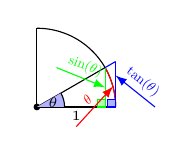
\begin{tikzpicture}
  %inner triangle
  \coordinate [] (A) at (0,0);
  \coordinate [] (B) at (0.866025403784,0);
  \coordinate [] (C) at (0.866025403784,0.5);

  \draw (1,0) arc[start angle=0, end angle=90, radius=1];
  \draw[red] (1,0) arc[start angle=0, end angle=30, radius=1];
  \draw[fill=black](0,0) circle (1 pt) node [above] {};
  \draw[](0,0) -- (1,0) node [midway,below,label={[label distance=-.30cm, font=\tiny]:{$1$}}] {};
  \draw[](0,0) -- (0,1) node [midway,below] {};

  \draw node[above] {} (A) -- node[below] {} (C);
  \draw [green] node[above] {} (B) -- node[below] {} (C);
  \draw [blue] node[below] {} (C) -- (1,0.57735026919);
  \draw [blue] (1,0) -- (1,0.57735026919);
  \draw [green,fill=green!30](0.766025403784,0) rectangle (0.866025403784,0.1);
  \draw [blue,fill=blue!30](.9,0) rectangle (1,0.1);
  \draw pic[draw,fill=blue!30,angle radius=10,"$\theta$",font=\tiny] {angle=B--A--C};    
  \draw [-latex, green] (.25,.5) -- (0.866025403784,0.25) node[above, sloped,midway,scale = .5] {sin($\theta$)};
  \draw [-latex, red] (.5,-.25) -- (0.96592582629,.2588190451) node[above, sloped,midway,scale = .5] {$\theta$};
  \draw [-latex, blue] (1.5,0) -- (1,.4) node[above, sloped,midway,scale = .5] {tan($\theta$)};


\end{tikzpicture}
\end{document}